\section{Results}
\label{s:results}
%Results; this should be a readable summary of the results from applying the approach. Don’t pursue death by figures but carefully select what visualisations (figures, tables) are functional for telling your story and logically lead to the main conclusions and policy advice?

% Convincing story, consistent with approach using carefully designed visuals and tables to support narrative
In this section, we summarise the key results from applying this approach, identifying the most robust policies for Gorssel, Deventer and Overijssel, and discussing options for synthesising policy choices between the three actors.


\subsection{Uncertainty Analysis}
Uncertainty Analysis revealed uncertainties in these ranges: x-y

The scenarios selected were based on understanding both how the policies perform under these uncertainty ranges, as well as under a diverse set of 'better' conditions. As such, the two 'worst case' scenarios fall within this uncertainty range, while the remaining scenarios fall across other ranges.


\subsection{Robust Decision Making}
%Look at the policies for the five different scenarios, and examine trade-offs using different robustness metrics.
For the robust decision making process two metrics were used: Satisficing (or the domain-criterion) and maximum regret. 
%#################################################################
%   REGRET AND SATISFICING - GORSSEL
%#################################################################
\subsubsection{Gorssel}
\textbf{Satisficing results} \newline
The results from this analysis: The results for Gorssels satisficing analysis with the domain criterion are shown in \autoref{fig:domain_criterion_gorsse}. The 12 selected policies are analysed for trade-offs and how satisficing their results are. \newline
Gorssels 'scenario 


\textbf{Regret results} \newline



\begin{figure}[H]
  \centering
  \begin{minipage}[b]{0.4\textwidth}
    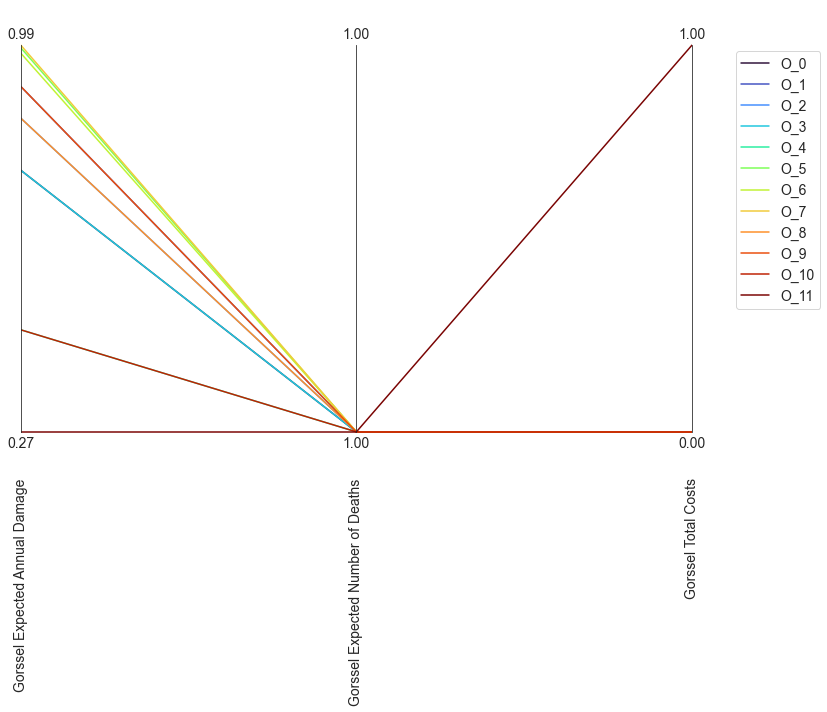
\includegraphics[width=1.15\textwidth]{report/figures/results/domain_criterion_Gorssel.png}
    \caption{Results for Gorssels domain criterion}
    \label{fig:domain_criterion_gorssel}
  \end{minipage}
  \hfill
  \begin{minipage}[b]{0.4\textwidth}
    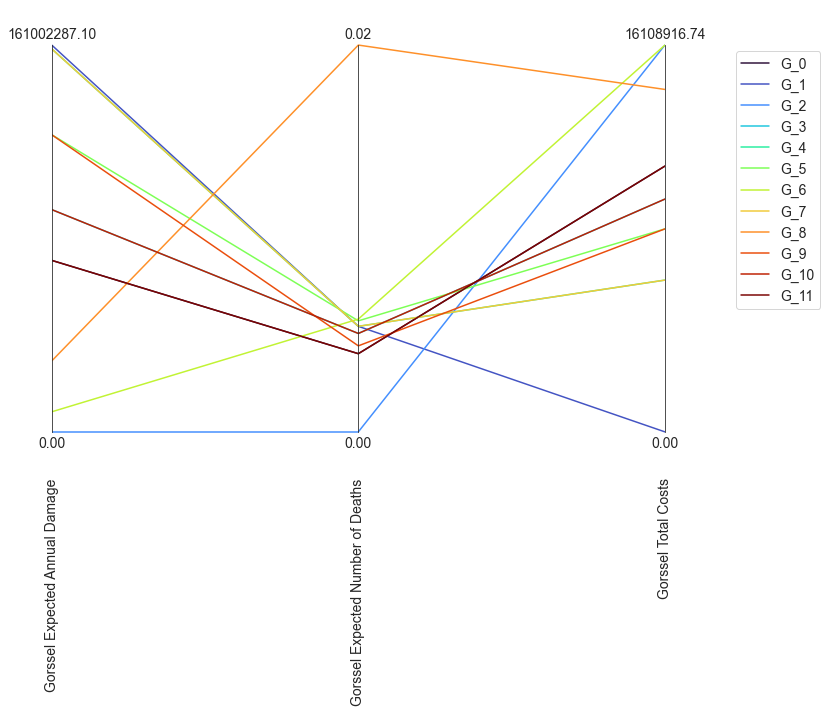
\includegraphics[width=1.15\textwidth]{report/figures/results/regret_figure_Gorssel.png}
    \caption{Results for Gorssel's maximum regret}
    \label{fig:regret_gorssel}
  \end{minipage}
\end{figure}




%#################################################################
%   REGRET AND SATISFICING - DEVENTER
%#################################################################
\subsubsection{Deventer}

\begin{figure}[H]
  \centering
  \begin{minipage}[b]{0.4\textwidth}
    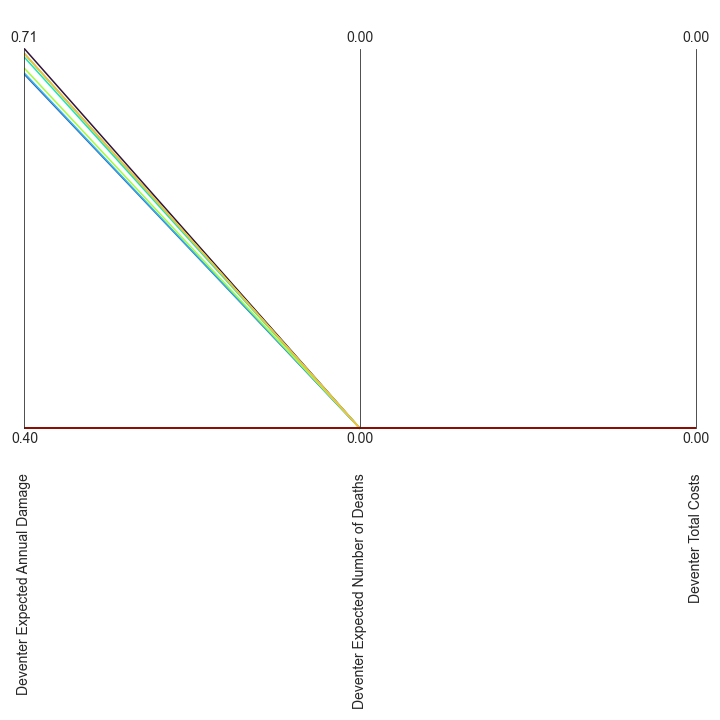
\includegraphics[width=1.15\textwidth]{report/figures/results/domain_criterion_Deventer.png}
    \caption{Results for Deventer's domain criterion}
    \label{fig:domain_criterion_Deventers}
  \end{minipage}
  \hfill
  \begin{minipage}[b]{0.4\textwidth}
    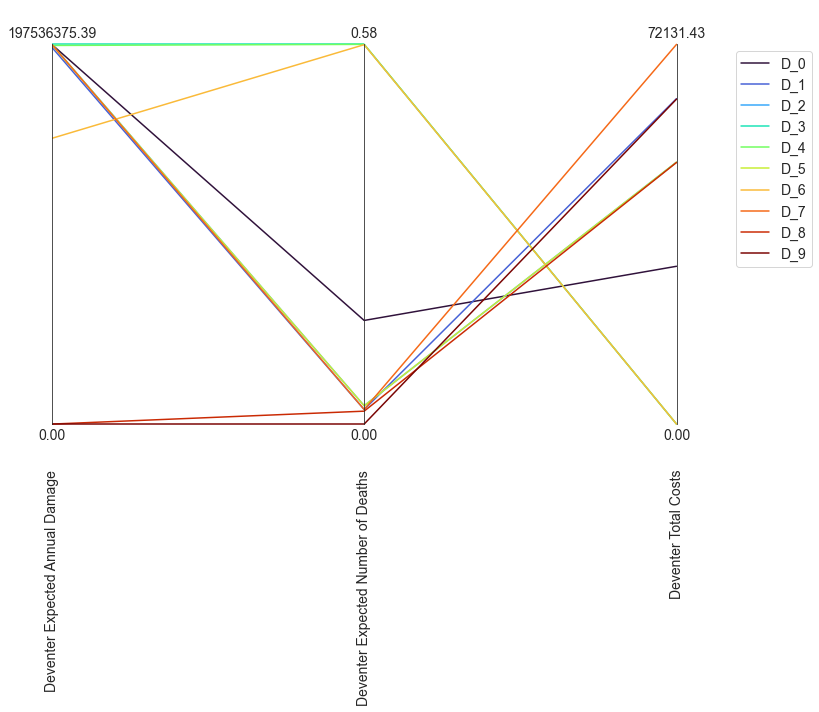
\includegraphics[width=1.15\textwidth]{report/figures/results/regret_figure_Deventer.png}
    \caption{Results for Deventer's maximum regret}
    \label{fig:regret_Deventers}
  \end{minipage}
\end{figure}

%#################################################################
%   REGRET AND SATISFICING - OVERIJSSEL
%#################################################################
\subsubsection{Overijssel}

\begin{figure}[H]
  \centering
  \begin{minipage}[b]{0.4\textwidth}
    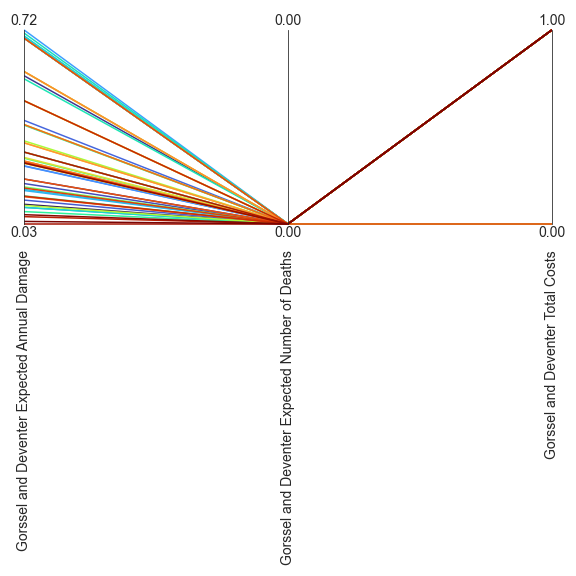
\includegraphics[width=1.15\textwidth]{report/figures/results/domain_criterion_Overijssel.png}
    \caption{Results for Overijssel's domain criterion}
    \label{fig:domain_criterion_Overijssels}
  \end{minipage}
  \hfill
  \begin{minipage}[b]{0.4\textwidth}
    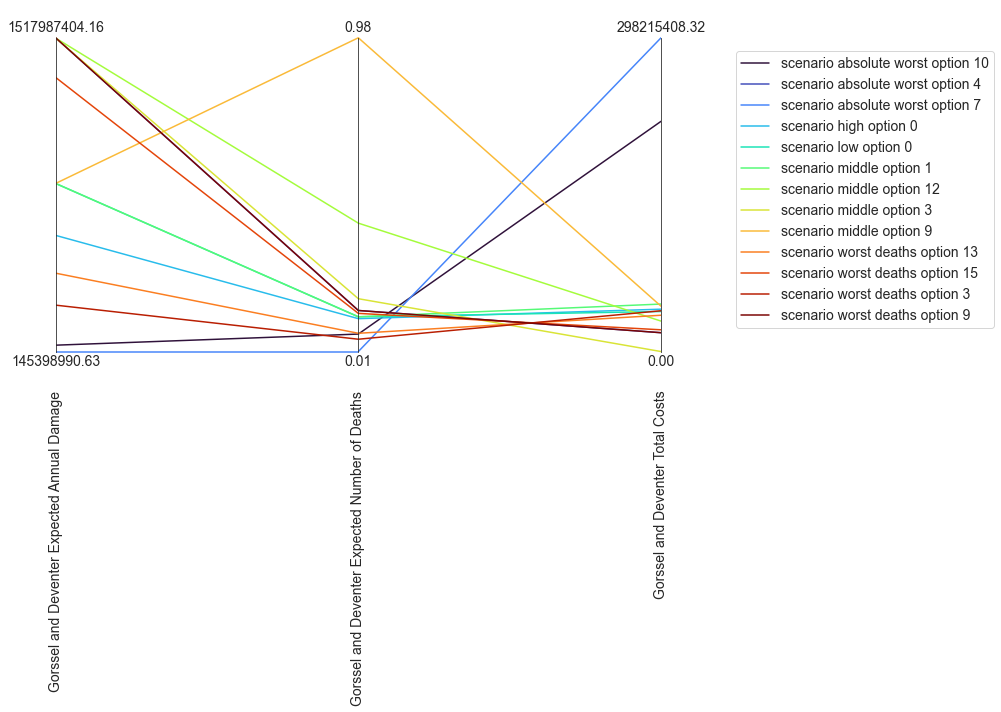
\includegraphics[width=1.15\textwidth]{report/figures/results/regret_figure_Overijssel.png}
    \caption{Results for Overijssels maximum regret}
    \label{fig:regret_Overijssels}
  \end{minipage}
\end{figure}

\subsection{Shortlisted Policies for each Actor}
From the robustness analysis, a subset of the top five most robust policies (prioritising regret-based metrics) were identified. Here, a brief description of each policy, and the relevant actions in terms of dike heightening, room the the river projects, and early warning systems are presented for each actor.
\subsubsection{Gorssel}
The five most robust policies for Gorssel are presented in Table
\begin{figure}[h]
    \centering
    \caption{-}
    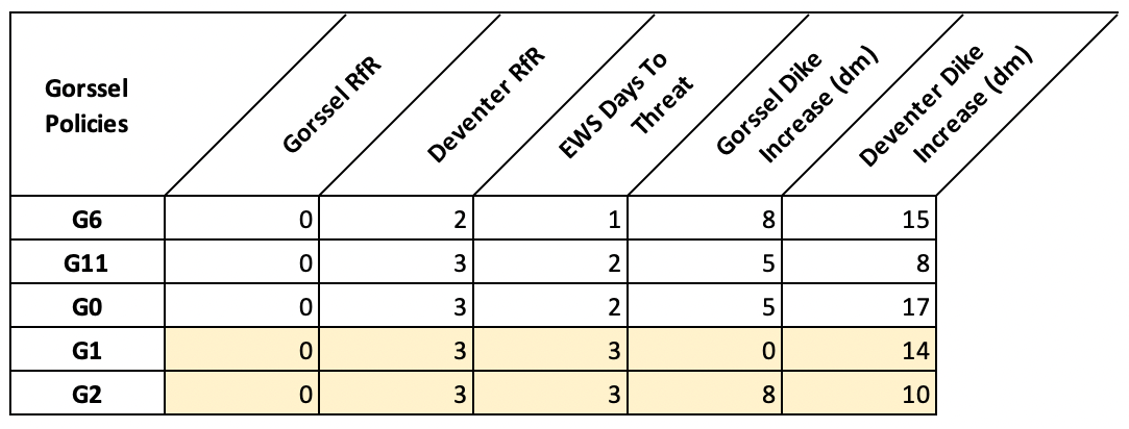
\includegraphics[width=0.4\textwidth]{report/figures/gpols.png}
    \label{fig:msmordm}
\end{figure}




\subsection{Sensitivity Analysis}

To see which policies and uncertainties have a large effect on model behaviour, a sensitivity analysis is carried out. The analysis of these can be viewed per actor in the following section. Firstly, the sensitivity analysis was done with feature scoring without the policies to get a grasp of which uncertainty the actors would be most sensitive to. After, policies are added and analysed to assess whether they would be sensitive or not. The generated figures for the sensitivity analysis can be found in Appendix \textbf{XXX}

\subsubsection{Gorssel}

From the sensitivity analysis for damage and deaths for Gorssel it becomes apparent that they are not only influenced by their own dike failure, but also by that of Deventer. This has to do with the fairness criteria specified by Gorssel, where they strive to achieve fairness between all actors in the Overijssel province. As a result, the failures of \textit{both} cities have the highest impact on the deaths and damage. When adding the policies, we observe that the sensitivity to dike failure remains the highest for both the deaths and damage. 

\subsubsection{Deventer}

For Deventer the biggest threat to damages and deaths is the dike failure of just Deventer. This is in line with expectations, because only their own dikes breaking would impact Deventer. And just as with Gorssel, we can observe that when adding the policies, we see that the outcome is still least robust under dike failure. 

\subsubsection{Overijssel}

For the costs of the province of Overijssel it can be observed that they are sensitive to dike increase. The sensitivity is biggest to dike increase in Gorssel, which is in line with reality as this is the most costly procedure in the province, other than Room for the River. However, because none of the policies for Overijssel recommend Room for the River, there is no observed sensitivity. Furthermore, the entire province shows a higher score on deaths and damages across the province as well when it comes to dike failure. 

\subsection{Policy Comparison}
Here, the top five policies from each actor are considered and compared to investigate opportunities for coalition forming, or to identify sources of tension in the policy-making process.